\documentclass[11pt, a4paper]{article}

\usepackage{graphicx}
\usepackage[english]{babel}
\usepackage[utf8x]{inputenc}
\usepackage{amsmath}
\usepackage{amssymb}
\usepackage{siunitx}
\usepackage{subfig}

\usepackage[a4paper,top=3cm,bottom=2cm,left=2cm,right=2cm,marginparwidth=1.75cm]{geometry}
\graphicspath{ {./images} }

\newcommand*{\qed}{\hfill\ensuremath{\quad\square}}%

\begin{document}

\setcounter{section}{2}
\section{Lecture 3 (17/02/2020)}
\subsection{Choice of coordinate system}
The choice of coordinate system should not affect the motion of an object. The coordinate system should be thought
off as a geometrical way of expressing a motion. The way in which the motion is expressed may differ but the motion
is still the same motion no matter how it is described. This is important since it builds intuition for describing
motion along a curve. This concept will be covered with an example below.\\
\\
\begin{figure}[h]
    \centerline{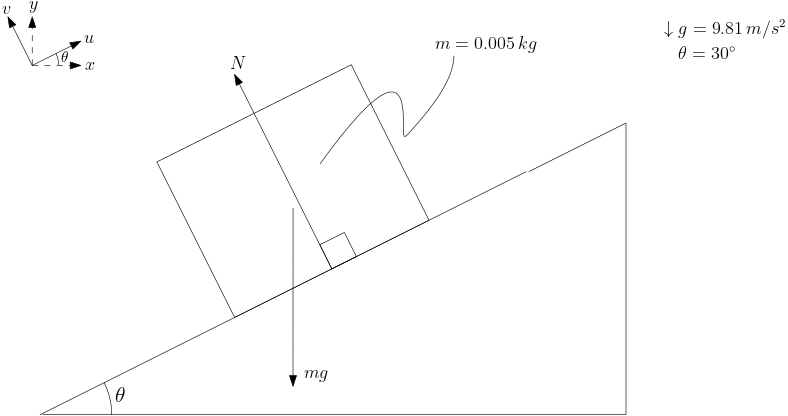
\includegraphics[width=10cm]{images/Crate_No_Friction.png}}
    \caption{The Free Body Diagram of the cup on a plane}
\end{figure}

Recall the example from lecture 1 with a cup on a table. The coordiante system for that problem was solved using 
the $u$- and $v$-axis which where offset from the $x$- and $y$-axis respectivly by an angle of $\theta$. The solution below
will solve the problem using the $x$- and $y$-axis.

\begin{gather}
    \Sigma F_x = N \cdot \sin(\theta) = m\ddot{x} \\
    \Sigma F_y = N \cdot \cos(\theta) - mg = m\ddot{y}
\end{gather}
There are now 3 variables and 2 equations making this system currently unsolvable. There needs to be another equation.
This equation based on some geometrical properties of the surface which can be seen in figure 2. 
Since the cup is moving along the surface we know the following:

\begin{figure}[h]
    \centerline{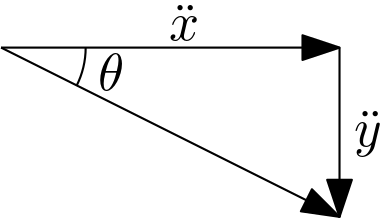
\includegraphics[width=3.5cm]{images/Vector_Sum.png}}
    \caption{The vector sum describing the relation between horizontal and vertical acceleration}
\end{figure}

\begin{gather}
    \tan(\theta) = \frac{\ddot{y}}{\ddot{x}} \Rightarrow \ddot{y} = \ddot{x} \tan(\theta)  
\end{gather}

Equation (3) being the constraint equation for this system introduces the 3rd and final equation needed for
solving this system.

\subsection{n,t-coordinates}
n,t-coordinates refers to normal, tangential coordinates. This is a coordinate system commonly used for describing
motion along curved surfaces and paths. It's important to note that this is in fact an inertial frame of reference. The
total displacement is always going to be 0 because of this since the coordinates move along with the object that
is being described.
\begin{figure}[h]
    \centerline{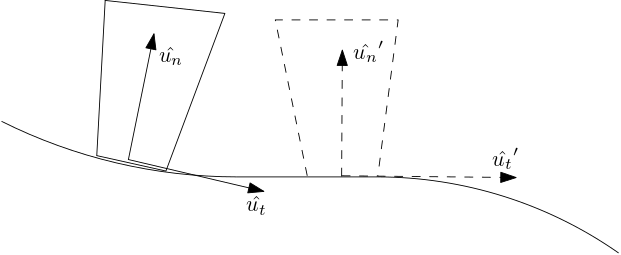
\includegraphics[width=10cm]{images/NT_example.png}}
    \caption{The movement of a cup along a curved surface}
\end{figure}

\begin{equation}
    \vec{v} = v_t \cdot \boldsymbol{\hat{u}_t} + 0 \cdot \boldsymbol{\hat{u}_n}
\end{equation}
Equation (4) describes the actual velocity of the object along the surface. Only the tangential component of the
force contributes to changes in velocity, and only the tangential component of the velocity vector describes
the velocity along the surface. It's worth knowing that this is all still expressed in a cartesian coordinate system.
the velocity vector $\vec{v}$ can also be described as $\vec{v} = v_x\boldsymbol{\hat{i}} + v_y\boldsymbol{\hat{j}}$.
By extension this means that the unit vectors $\boldsymbol{\hat{u}_t}$ and $\boldsymbol{\hat{u}_n}$ are also vectors expressed in cartesian coordinates.

\subsection{derrivation for motion along a curved path}
The acceleration vector $\vec{a}$ is considered a type of constraint equation for the movement, 
since the object has to move along the curved path. Applying the product rule gives the following:

\begin{gather}
    a = \frac{dv}{dt} \Rightarrow \vec{a} = \frac{d(v_t \cdot \boldsymbol{\hat{u}})}{dt} = \frac{dv}{dt} \cdot 
        \boldsymbol{\hat{u}} + v_t \frac{d\boldsymbol{\hat{u}}}{dt}
\end{gather}

Consider the following: a point mass moves an infetesimal distance $ds$\footnote{Since all values for the differential element are very small
$ds$ is approximated to do be straight eventhough it is technically curved very slightly.} along a curved path.
This means the angle $\phi$ increases with $d\phi$. The radius of curvature will be $\rho$. Figure 4 shows the geometrical relation.
\begin{figure}[h]
    \centerline{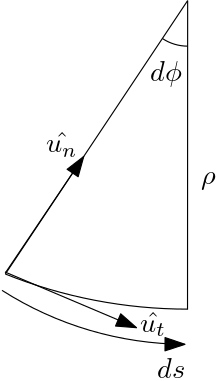
\includegraphics[width=3.5cm]{images/Differential_element.png}}
    \caption{A differential element of an object moving along a curved path}
\end{figure}
Since the increases in angle are small,
which is to say, way less then 1 a first order Taylor expansion can be used to approximate the value:

\begin{gather}
    T(x) = \sum_{n=0}^{\infty} \frac{f^{(n)}(a)}{n!} (x-a)^n \quad\text{for}\quad f(x) = \sin(x) \quad \text{at a=0}\\
    T_1(x) = 0 + \frac{\cos(0)}{1} (x-0) = x\\
    \sin(x) \approx x \qed
\end{gather}

Because of this property we can determine the following:

\begin{gather}
    ds = \rho d\phi\\
    d\phi = \frac{ds}{\rho}
\end{gather}

\begin{figure}[h]
    \centerline{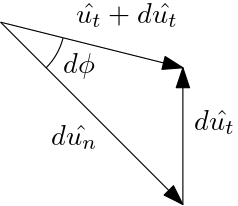
\includegraphics[width=3.5cm]{images/Differential element_2.png}}
    \caption{The geometrical relation between $d\boldsymbol{{\hat{u}_n}}$, $d\boldsymbol{{\hat{u}_t}}$ and $d\phi$}
\end{figure}
From figure 5 we can see that:
\begin{gather}
    d\boldsymbol{\hat{u}_t} = d\phi \cdot \boldsymbol{\hat{u}_n}
\end{gather}

Using equation (10) and (11) and taking the derrivative with respect to time we can see that:
\begin{gather}
    \frac{\boldsymbol{\hat{u}_t}}{dt} = \frac{\frac{ds}{\rho} \cdot \boldsymbol{\hat{u}_n}}{dt} =
        \frac{ds}{dt} \cdot \frac{1}{\rho} \cdot \boldsymbol{\hat{u}_n}
\end{gather}

Equation (12) can then be simplified further to the following:
\begin{gather}
    \vec{a} = a_t \cdot \boldsymbol{\hat{u}_t} + \frac{v_t^2}{\rho}\cdot \boldsymbol{\hat{u}_n}
\end{gather}
Equation (13) is now in practical, usuable form for calculations.

\newpage
\subsection{Examples with n,t-coordinates 1}
\begin{figure}[h]
    \centerline{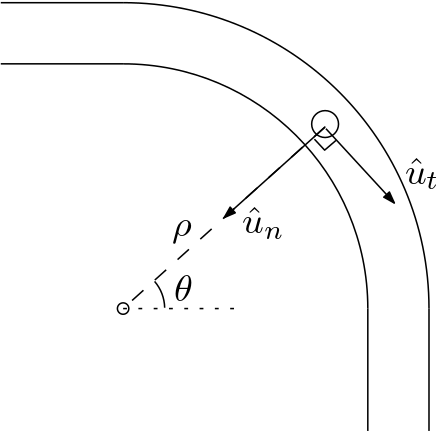
\includegraphics[width=3.5cm]{images/NT_example_2.png}}
    \caption{Representation of the problem, let $\rho=100\,m$, $v_t=5\,m/s$ and $a_t=1\,m/s^2$}
\end{figure}

\begin{gather}
    \vec{a} = a_t \boldsymbol{\hat{u}_t} + a_n \boldsymbol{\hat{u}_n}\\
    \boldsymbol{\hat{u}_t} =  \begin{pmatrix} \cos(\ang{45})\\ -\sin(\ang{45}) \end{pmatrix} =
        \begin{pmatrix} \frac{1}{2}\sqrt{2} \\ -\frac{1}{2}\sqrt{2}\end{pmatrix} =
        \frac{1}{2}\sqrt{2} \, \boldsymbol{\hat{i}} - \frac{1}{2}\sqrt{2} \, \boldsymbol{\hat{j}}\\
    \boldsymbol{\hat{u}_n} =  \begin{pmatrix} -\cos(\ang{45})\\ -\sin(\ang{45}) \end{pmatrix} =
        \begin{pmatrix} -\frac{1}{2}\sqrt{2} \\ -\frac{1}{2}\sqrt{2}\end{pmatrix} =
        -\frac{1}{2}\sqrt{2} \, \boldsymbol{\hat{i}} - \frac{1}{2}\sqrt{2} \, \boldsymbol{\hat{j}}
\end{gather}
The unit vectors $\boldsymbol{\hat{u}_t}$ and $\boldsymbol{\hat{u}_n}$ represent the direction of the components
of the acceleration and velocity vector. $\boldsymbol{\hat{u}_t}$ is tangential to the rotation and $\boldsymbol{\hat{u}_n}$
is towards the center of the curve.

Using this information:
\begin{gather}
    a_n = \frac{v_t^2}{\rho} = \frac{(5\,m/s)^2}{100\,m} = 0.25\,m/s^2
\end{gather}

\subsection{Example with n,t-coordiantes 2}
In 3D the n,t-coordinates gain an extra component. This component is perpendicular to both the 
normal and tangential vector, and is reffered to as the bionomial vector. The following example
deals with a problem in 3D which is reduced to two 2-dimensional problems to solve. 3-dimensional
dynamics is outside the scope of the course\footnote{WB1135, TU Delft} and will be covered in advanced Dynamics in year 2 quarter 1.\\
\\
\begin{figure}[h]
    \centering
    \subfloat[Top view]{{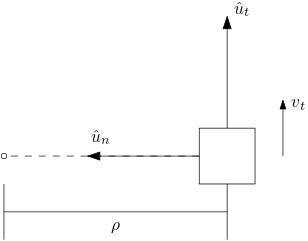
\includegraphics[width=5cm]{images/Top_View.png}}}%
    \qquad
    \subfloat[Front View]{{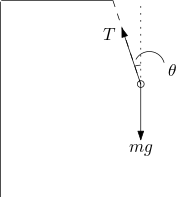
\includegraphics[width=3.5cm]{images/Front_View.png}}}%
    \caption{The problem reduced to two 2-dimensional, easier to solve situations}
\end{figure}

Looking at the 2D simplification of the problem from above shows a very typical circular motion.
The distance $\rho$ is the distance to the circle around which the mass rotates, and perpendicular 
to that the tangential component pointing in the direction of rotation. Figure 7 Shows the Free body diagram of the problem when
observed from the front in (b) and the top in (a). From here it is possible to determine the equations of motion.

\begin{gather}
    \Sigma F_x = -\sin(\theta)\cdot T = m\ddot{x}\\
    \ddot{x} = -a_n = -\frac{v_t^2}{\rho}
\end{gather}

After this it's a fairly typical solution solving for the value of T.

\subsection{Example with unknown radius of curvature}
In some case a problem presents a curved surface, where the radius of curvature 
$\rho$ is not known or not constant. Since the surface is often curved as some function of $x$ the
radius of curvature can also be computed as a function of $x$. This can be done with
the following equation:

\begin{gather}
    \rho = \frac{(1+(\frac{dy}{dx})^2)^\frac{3}{2}}{\frac{d^2y}{dx^2}}
\end{gather}
The following example follows a problem where the the curved surface is a function of $x$.\\
\\
\begin{figure}[h]
    \centerline{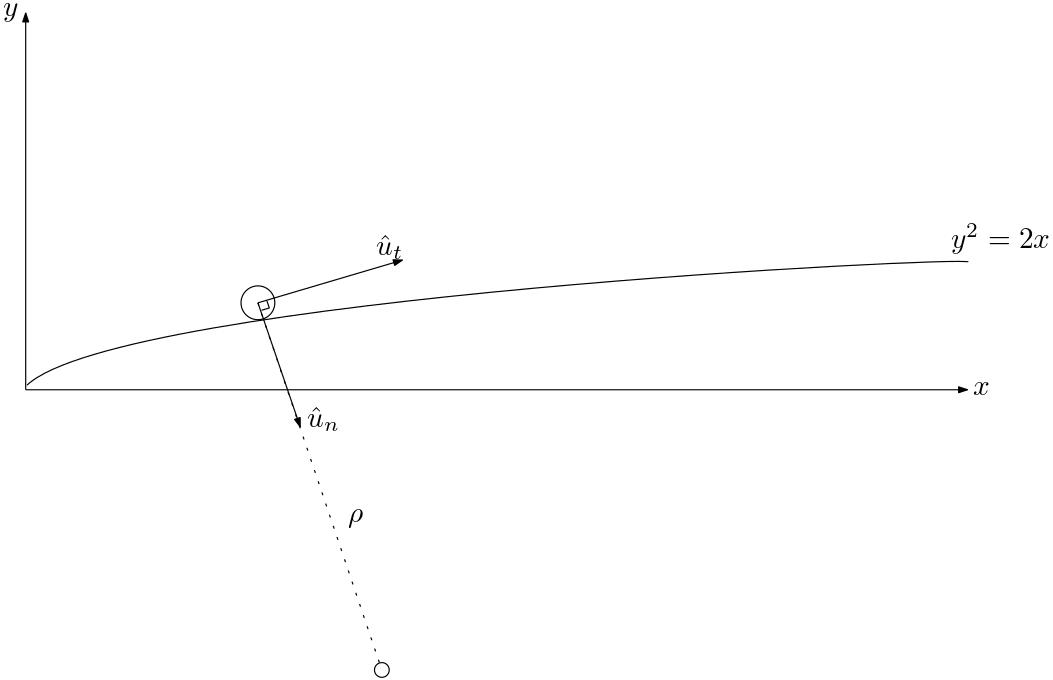
\includegraphics[width=10cm]{images/Final_example.png}}    
    \caption{Curved surface $y$ as a function of $x$}
\end{figure}

\begin{gather}
    y^2 = 2x \Rightarrow y = \sqrt{2x}\\
    \frac{dy}{dx} = \frac{\sqrt{2}}{2\sqrt{x}}\\
    \frac{d^2y}{dx^2} = \frac{-\sqrt{2}}{4x\sqrt{x}}
\end{gather}
Subsituting equations (22) and (23) into (20) and simplifying gives the following:
\begin{equation}
    \rho = \frac{-4x\sqrt{x}-2\sqrt{x}\sqrt{1+\frac{1}{2x}}}{\sqrt{2}}    
\end{equation}
This equation determins the radius of curvature $\rho$ at any point $x$ along the curve.

\end{document}
